\documentclass[unicode,11pt,a4paper,oneside,numbers=endperiod,openany]{scrartcl}

% Required package
\usepackage{amssymb}
\usepackage{graphicx}
\usepackage{amsmath}
\usepackage{matlab-prettifier}
\usepackage{float}
\usepackage[export]{adjustbox}
\usepackage{multirow}
\usepackage{booktabs}
\usepackage{amsthm} % math theorems
\usepackage{ifthen}
\usepackage{physics} % responsive norm, abs, ...
\usepackage{algorithm}
\usepackage{algpseudocode}
\usepackage{array} % for table
\usepackage{mathtools} % for \coloneq
\usepackage{xcolor, soul} % highlight

\renewcommand{\thesubsection}{\arabic{subsection}}

\newtheorem{theorem}{Theorem}[section]
% 1: title, 2: label, 3: content
\newcommand{\myth}[3]{
    \begin{theorem}[#1] 
        \label{#2} 
        #3 
    \end{theorem}
}

% 1: color, 2: content
\newcommand{\mathcolorbox}[2]{\colorbox{#1}{\(\displaystyle #2\)}}

% 1: if numbered equation, 2: label, 3: content
\newcommand{\myex}[3]{
    \ifthenelse{\equal{#1}{true}}{
        \begin{equation} \label{#2} \begin{aligned} #3 \end{aligned} \end{equation}
    }{
        \begin{equation*} \label{#2} \begin{aligned} #3 \end{aligned} \end{equation*}
    }
}

% vector shortcut
\newcommand{\myvec}[1]{\begin{bmatrix} #1 \end{bmatrix}}

% 1: letter of vector, 2: 
\newcommand\vibar[2]{\mathbf{\overline{#1}}_#2}

% 1: caption, 2: label, 3: trim, 4: figure within figures folder
\newcommand{\myfigure}[4]{
    \begin{figure}[htbp]
    \centering
    \caption{#1}
    \label{#2}
    \includegraphics[width=\paperwidth, trim=#3]{./figures/#4}
    \end{figure}
}

\def\ex2f{f(\mathbf{x}^*)}

\usepackage{ifthen}
\usepackage[utf8]{inputenc}
\usepackage{graphics}
\usepackage{graphicx}
\usepackage{hyperref}
\usepackage{amsmath}

\pagestyle{plain}
\voffset -5mm
\oddsidemargin  0mm
\evensidemargin -11mm
\marginparwidth 2cm
\marginparsep 0pt
\topmargin 0mm
\headheight 0pt
\headsep 0pt
\topskip 0pt        
\textheight 255mm
\textwidth 165mm

\newcommand{\duedate} {}
\newcommand{\setduedate}[1]{%
\renewcommand\duedate {\textbf{Due date:}~ #1}}
\newcommand\isassignment {false}
\newcommand{\setassignment}{\renewcommand\isassignment {true}}
\newcommand{\ifassignment}[1]{\ifthenelse{\boolean{\isassignment}}{#1}{}}
\newcommand{\ifnotassignment}[1]{\ifthenelse{\boolean{\isassignment}}{}{#1}}

\newcommand{\assignmentpolicy}{
\begin{table}[h]
\begin{center}
\scalebox{0.8} {%
\begin{tabular}{|p{0.02cm}p{16cm}|}
\hline
&\\
\multicolumn{2}{|c|}{\Large\textbf{Numerical Computing 2023 ---  Submission Instructions}}\\
\multicolumn{2}{|c|}{\large\textbf{(Please, notice that following instructions are mandatory: }}\\
\multicolumn{2}{|c|}{\large\textbf{submissions that don't comply with, won't be considered)}}\\
&\\
\textbullet & Assignments must be submitted to \href{https://www.icorsi.ch/course/view.php?id=14666}{iCorsi} (i.e. in electronic format).\\
\textbullet & Provide both executable package and sources (e.g. C/C++ files, MATLAB). 
If you are using libraries, please add them in the file. Sources must be organized in directories called:\\
\multicolumn{2}{|c|}{\textit{Project\_number\_lastname\_firstname}}\\
& and  the  file must be called:\\
\multicolumn{2}{|c|}{\textit{project\_number\_lastname\_firstname.zip}}\\
\multicolumn{2}{|c|}{\textit{project\_number\_lastname\_firstname.pdf}}\\
\textbullet &  The TAs will grade your project by reviewing your project write-up, and looking at the implementation you attempted, and benchmarking your code's performance.\\

\textbullet & You are allowed to discuss all questions with anyone you like; however: (i) your submission must list anyone you discussed problems with and (ii) you must write up your submission independently.\\
\hline
\end{tabular}
}
\end{center}
\end{table}
}
\newcommand{\punkte}[1]{\hspace{1ex}\emph{\mdseries\hfill(#1~\ifcase#1{Points}\or{Points}\else{Points}\fi)}}


\newcommand\serieheader[6]{
\thispagestyle{empty}%
\begin{flushleft}

\includegraphics[width=0.45\textwidth]{CI_logo}
\end{flushleft}
  \noindent%
  {\large\ignorespaces{\textbf{#1}}\hspace{\fill}\ignorespaces{ \textbf{#2}}}\\ \\%
  {\large\ignorespaces #3 \hspace{\fill}\ignorespaces #4}\\
  \noindent%
  \bigskip
  \hrule\par\bigskip\noindent%
  \bigskip {\ignorespaces {\Large{\textbf{#5}}}
  \hspace{\fill}\ignorespaces \large \ifthenelse{\boolean{\isassignment}}{\duedate}{#6}}
  \hrule\par\bigskip\noindent%  \linebreak
 }

\makeatletter
\def\enumerateMod{\ifnum \@enumdepth >3 \@toodeep\else
      \advance\@enumdepth \@ne
      \edef\@enumctr{enum\romannumeral\the\@enumdepth}\list
      {\csname label\@enumctr\endcsname}{\usecounter
        {\@enumctr}%%%? the following differs from "enumerate"
	\topsep0pt%
	\partopsep0pt%
	\itemsep0pt%
	\def\makelabel##1{\hss\llap{##1}}}\fi}
\let\endenumerateMod =\endlist
\makeatother




\usepackage{textcomp}





\begin{document}

\setassignment
\setduedate{Thursday, 3 October 2024, 23:59}

\serieheader
{Discrete Mathematics}
{2024}
{%
\textbf{Student:} Jeferson Morales Mariciano 
\href{mailto:jmorale@ethz.ch}{\(<\)jmorale@ethz.ch\(>\)} \\\\}
{\vspace{-1cm}}%\textbf{Discussed with:} }
{Assignment 2}{}

%----------------------------------------------------------------------------------
\section{Exercise 2.3, Simplifying a Formula (\(\star\)) \hfill (8 Points)}

Consider the propositional formula

\[
F = \left( (B \lor C) \to ((A \lor \neg B) \land C) \right) \lor (A \land \neg C)
\]

\noindent Give a formula \( G \) that is equivalent to \( F \), but in which each atomic formula \( A \), \( B \), and \( C \)
appears at most once. Prove that \( F \equiv G \) by providing a sequence of equivalence transformations 
with \textit{at most} 12 steps.

\noindent \textbf{Expectation.} 
Your proof should be in the form of a sequence of steps, where each step
consists of applying the definition of \( \to \) 
(that is \( F \to G \equiv \neg F \lor G \)), 
one of the rules given in Lemma 2.1 of the lecture notes 
\footnote{Lemma 2.1 states rules involving propositional symbols, 
but you may apply those rules at the level of formulas 
(see Section 2.3.5 of the lecture notes).}, 
or one of the following rules: 
\( F \land \neg F \equiv \bot \), 
\( F \land \bot \equiv \bot \), 
\( F \lor \bot \equiv F \), 
\( F \lor \neg F \equiv \top \), 
\( F \land \top \equiv F \), 
and \( F \lor \top \equiv \top \). 
For this exercise, associativity is to be applied as in Lemma 2.1.3. 
Each step of your proof should apply a \textit{single} rule \textit{once} 
and state \textit{which} rule was applied.
\\\newline

The following 12 steps show the equivalence between \( F \) and \( G \), 
where \( G  \coloneq \neg B \lor A \).

\myex{}{ex2-3-proof}{
F &= \left( 
        \left(B \lor C \right) \rightarrow \left( \left(A \lor \neg B \right) \land C \right) 
    \right) 
    \lor \left( A \land \neg C \right) \\
F &= \left( 
        \mathcolorbox{yellow}{\neg \left(B \lor C \right) \lor \left( \left( A \lor \neg B \right) \land C \right)} 
    \right) 
    \lor \left( A \land \neg C \right) 
&&&&&&&&&& \text{def of \(\rightarrow\)} \\
F &= \left( 
        \mathcolorbox{yellow}{\left( \neg B \land \neg C \right)} \lor \left( \left(A \lor \neg B \right) \land C \right) 
    \right) 
    \lor \left( A \land \neg C \right)
&&&&&&&&&& \text{def De Morgan} \\
F &= \left( 
        \left( \neg B \land \neg C \right) 
        \lor \mathcolorbox{yellow}{\left( C \land \left( A \lor \neg B \right) \right)}
    \right)
    \lor \left( A \land \neg C \right)
&&&&&&&&&& \text{def commutative} \\
F &= \left( 
        \left( \neg B \land \neg C \right) 
        \lor \mathcolorbox{yellow}{\left( C \land A \right) \lor \left( C \land \neg B \right)}
    \right)
    \lor \left( A \land \neg C \right)
&&&&&&&&&& \text{def 1st distributive law} \\
F &= \left( 
        \left( \neg B \land \neg C \right) 
        \lor \mathcolorbox{yellow}{\left( C \land \neg B \right) \lor \left( C \land A \right)}
    \right)
    \lor \left( A \land \neg C \right)
&&&&&&&&&& \text{def commutative} \\
F &= \left( 
        \mathcolorbox{yellow}{
            \left( \neg B \land \left( C \lor \neg C \right) \right)  
        }
        \lor \left( C \land A \right)
    \right)
    \lor \left( A \land \neg C \right)
&&&&&&&&&& \text{def 1st distributive law} \\
F &= \left( 
        \mathcolorbox{yellow}{
            \left( \neg B \land \top \right)  
        }
        \lor \left( C \land A \right)
    \right)
    \lor \left( A \land \neg C \right)
&&&&&&&&&& F \lor \neg F \equiv \top \\
F &= \left( 
        \mathcolorbox{yellow}{\neg B}
        \lor \left( C \land A \right)
    \right)
    \lor \left( A \land \neg C \right)
&&&&&&&&&& F \land \top \equiv F \\
F &= \neg B 
    \lor \left(
    \mathcolorbox{yellow}{
        \left( C \land A \right) \lor \left( A \land \neg C \right)
    }
    \right)
&&&&&&&&&& \text{def associativity} \\
F &= \neg B 
    \lor \left(
    \mathcolorbox{yellow}{
        A \land \left( C \lor \neg C \right)
    }
    \right)
&&&&&&&&&& \text{def 1st distributive law}  \\
F &= \neg B 
    \lor \left(
    \mathcolorbox{yellow}{
        A \land \top
    }
    \right)
&&&&&&&&&& F \lor \neg F \equiv \top \\
F &= \neg B \lor \mathcolorbox{yellow}{A}
&&&&&&&&&& F \land \top \equiv F \\
}

Finally, for the formula \( G \) defined as \( G \coloneq \neg B \lor A \),
we have shown that \( F \equiv G \) by applying a 12-step sequence of equivalence transformations.


% We define two binary logical operators \( \heartsuit \) and \( \diamondsuit \) as follows:

% \begin{center}
% \begin{minipage}{0.3\textwidth}

% \[
% \begin{array}{c|c||c}
% A & B & A \heartsuit B \\
% \hline
% 0 & 0 & 1 \\
% 0 & 1 & 0 \\
% 1 & 0 & 1 \\
% 1 & 1 & 1 \\
% \end{array}
% \]

% \end{minipage}
% \begin{minipage}{0.3\textwidth}

% \[
% \begin{array}{c|c||c}
% A & B & A \diamondsuit B \\
% \hline
% 0 & 0 & 1 \\
% 0 & 1 & 0 \\
% 1 & 0 & 0 \\
% 1 & 1 & 1 \\
% \end{array}
% \]

% \end{minipage}
% \end{center}

% \subsection*{a) (\(\star\))}  
% Are \(\heartsuit\) and \(\diamondsuit\) commutative, i.e., does it hold

% \[
% A \heartsuit B \equiv B \heartsuit A 
% \quad \text{and} \quad 
% A \diamondsuit B \equiv B \diamondsuit A ?
% \]

% \noindent Argue by comparing function tables.
% \\\newline

% Let's compare the function tables of the \( \heartsuit \) operator to check commutativity,

% \[
% \begin{array}{c|c}
% A \heartsuit B & B \heartsuit A \\
% \hline
% 1 & 1 \\
% \textcolor{red}{0} & \textcolor{red}{1} \\
% \textcolor{red}{1} & \textcolor{red}{0} \\
% 1 & 1 \\
% \end{array}
% \]

% The function tables are not equivalent, i.e. \( A \heartsuit B \not\equiv B \heartsuit A \),
% because the \( \heartsuit \) operator has an ordering dependency on the propositional symbols:
% only when the left propositional symbol is false, the result is false.
% That's why when swapping the order of the symbols for the operators, 
% the function tables are not equivalent.
% E.g. for \( A = 0 \) and \( B = 1 \), \( A \heartsuit B = 0 \) and \( B \heartsuit A = 1 \),
% hence \underline{not commutative}.
% \\

% Afterwards, let's compare the function tables of the \( \diamondsuit \) operator 
% to check commutativity,   

% \[
% \begin{array}{c|c}
% A \diamondsuit B & B \diamondsuit A \\
% \hline
% 1 & 1 \\
% 0 & 0 \\
% 0 & 0 \\
% 1 & 1 \\
% \end{array}
% \]

% The function tables are equivalent, i.e. \( A \diamondsuit B \equiv B \diamondsuit A \),
% because the \( \diamondsuit \) operator has no ordering dependency on the propositional symbols:
% swapping the order of the symbols for the operators does not change the function tables.
% E.g. for \( A = 0 \) and \( B = 1 \), \( A \diamondsuit B = 0 \) and \( B \diamondsuit A = 0 \),
% hence \underline{commutative}.


% \subsection*{b) (\(\star\))} 
% Prove or disprove that

% \[
% (\neg A \heartsuit B) \diamondsuit (B \diamondsuit C) 
% \equiv 
% \neg(A \diamondsuit B) \heartsuit \neg(A \diamondsuit C)
% \]

% \noindent by computing and comparing the function tables of the left-hand-side 
% and the right-hand-side formulas.
% \\\newline

% From the function table of the 3 propositional symbols \( A \), \( B \), and \( C \),

% \[
% \begin{array}{c|c|c}
% A & B & C \\
% \hline
% 0 & 0 & 0 \\
% 0 & 0 & 1 \\
% 0 & 1 & 0 \\
% 0 & 1 & 1 \\
% 1 & 0 & 0 \\
% 1 & 0 & 1 \\
% 1 & 1 & 0 \\
% 1 & 1 & 1 \\
% \end{array}
% \]

% we compute the left-hand-side formula as follows,

% \[
% \begin{array}{c|c|c|c}
% \neg A 
% & \neg A \heartsuit B 
% & B \heartsuit C 
% & (\neg A \heartsuit B) \diamondsuit (B \heartsuit C) \\
% \hline
% 1 & 1 & 1 & 1 \\
% 1 & 1 & 0 & 0 \\
% 1 & 1 & 1 & 1 \\
% 1 & 1 & 1 & 1 \\
% 0 & 1 & 1 & 1 \\
% 0 & 1 & 0 & 0 \\
% 0 & 0 & 1 & 0 \\
% 0 & 0 & 1 & 0 \\
% \end{array}
% \]

% and the right-hand-side formula as follows,

% \[
% \begin{array}{c|c|c|c|c}
% A \diamondsuit B 
% & \neg (A \diamondsuit B) 
% & A \diamondsuit C 
% & \neg (A \diamondsuit C) 
% & \neg (A \diamondsuit B) \heartsuit \neg (A \diamondsuit C) \\
% \hline
% 1 & 0 & 1 & 0 & 1 \\
% 1 & 0 & 0 & 1 & 0 \\
% 0 & 1 & 1 & 0 & 1 \\
% 0 & 1 & 0 & 1 & 1 \\
% 0 & 1 & 0 & 1 & 1 \\
% 0 & 1 & 1 & 0 & 1 \\
% 1 & 0 & 0 & 1 & 0 \\
% 1 & 0 & 1 & 0 & 1 \\
% \end{array}
% \]

% by comparing the left-hand-side and right-hand-side function tables, 
% we can see that \underline{they are not equivalent}, i.e. 

% \[
% \begin{array}{c|c}
% (\neg A \heartsuit B) \diamondsuit (B \diamondsuit C) 
% & \neg(A \diamondsuit B) \heartsuit \neg(A \diamondsuit C) \\
% \hline
% 1 & 1 \\
% 0 & 0 \\
% 1 & 1 \\
% 1 & 1 \\
% 1 & 1 \\
% \textcolor{red}{0} & \textcolor{red}{1} \\
% 0 & 0 \\
% \textcolor{red}{0} & \textcolor{red}{1} \\
% \end{array}
% \]

% \[
% (\neg A \heartsuit B) \diamondsuit (B \diamondsuit C) 
% \not\equiv 
% \neg(A \diamondsuit B) \heartsuit \neg(A \diamondsuit C)
% \]

    
% \subsection*{c) (\(\star \star\))} 
% Let \( F \) be a formula with the following function table:

% \[
% \begin{array}{c|c|c||c}
% A & B & C & F \\
% \hline
% 0 & 0 & 0 & 1 \\
% 0 & 0 & 1 & 1 \\
% 0 & 1 & 0 & 1 \\
% 0 & 1 & 1 & 0 \\
% 1 & 0 & 0 & 1 \\
% 1 & 0 & 1 & 1 \\
% 1 & 1 & 0 & 0 \\
% 1 & 1 & 1 & 1 \\
% \end{array}
% \]

% \noindent Find a formula \( G \) containing only the logical operators \(\heartsuit\) and \(\diamondsuit\), 
% in which the propositional symbols \( A \), \( B \), and \( C \) all appear exactly once, 
% and such that \( G \equiv F \). 
% No justification is required.
% \\\newline

% Let \( G \) be defined as \( G \coloneq (C \diamondsuit A) \heartsuit B \).
% Then, the function table of \( G \) is as follows,

% \[
% \begin{array}{c|c}
% C \diamondsuit A & (C \diamondsuit A) \heartsuit B \\
% \hline
% 1 & 1 \\
% 0 & 1 \\
% 1 & 1 \\
% 0 & 0 \\
% 0 & 1 \\
% 1 & 1 \\
% 0 & 0 \\
% 1 & 1 \\
% \end{array}
% \longrightarrow
% \begin{array}{c|c}
% G & F \\
% \hline
% 1 & 1 \\
% 1 & 1 \\
% 1 & 1 \\
% 0 & 0 \\
% 1 & 1 \\
% 1 & 1 \\
% 0 & 0 \\
% 1 & 1 \\
% \end{array}
% \]

% by comparing the function tables of \( F \) and \( G \), 
% we can see that \( G \equiv F \). 
% All constraints are satisfied: only logical operators \( \heartsuit, \diamondsuit \)
% and propositional symbols \( A, B, C \) appear exactly once.


% Consider the quadratic function \( f: \mathbb{R}^2 \rightarrow \mathbb{R} \) defined as:

% \myex{true}{eq:ex1-f}{
%     f(\mathbf{x}) = 7 x^2 + 4 xy + y^2
% }

% \noindent where \( \mathbf{x} = (x, y)^T \).

% \begin{enumerate}
%     \item Write this function in canonical form, i.e.
%           \( f( \mathbf{x} ) = \frac{1}{2} \mathbf{x}^T \mathbf{A} \mathbf{x} + \mathbf{b}^T \mathbf{x} + c \),
%           where \( A \) is a symmetric matrix.

%     \item Describe briefly how the Conjugate Gradient (CG) Method works
%           and discuss whether it is suitable to minimize \( f \) from equation \ref{eq:ex1-f}.
%           Explain your reasoning in detail (max. 30 lines).
% \end{enumerate}

% \subsection{Answer}

% The function written in canonical form corresponds to:

% \myex{false}{eq:ex1-f-quadratic}{
%     f( \mathbf{x} )
%     &= 7 x^2 + 4 xy + y^2 \\
%     &= \myvec{7x + 2y & 2x + y} \myvec{x \\ y} \\
%     &= \myvec{x & y} \myvec{7 & 2 \\ 2 & 1} \myvec{x \\ y} \\
%     &= \frac{1}{2} \myvec{x & y} \myvec{14 & 4 \\ 4 & 2} \myvec{x \\ y} \\
%     &= \frac{1}{2} \mathbf{x}^T \mathbf{A} \mathbf{x}
% }

% \noindent With \( \mathbf{b} = \mathbf{0}, \; c = 0 \),
% and \( A \) being clearly a symmetric matrix:

% \myex{false}{}{
%     \mathbf{A} = \myvec{14 & 4 \\ 4 & 2}
% }

% \noindent Let's verify if \( A \) is positive define as required by the quadratic form:

% \myex{false}{}{
%     \det \left( \lambda I - \mathbf{A} \right)
%     &= \mdet{\lambda - 14 & -4 \\ -4 & \lambda - 2} \\
%     &= \lambda^2 - 16 + 12 \\
%     &\Rightarrow \lambda_{1,2} = 8 \pm 2 \sqrt{13} > 0
% }

% \noindent Finally, since all eigenvalues are positive, \( \mathbf{A} \) is SPD.

% \subsection{Answer}

% The CG method is an iterative algorithm for solving a linear system of equations
% \( A x = b \) where \( A \in \mathbb{R}^{n \times n} \) is a \textbf{symmetric positive definite} matrix.
% For (\ref{eq:ex1-f}) we proved that \( A \) is SPD, which already perfectly fits the requirements.
% The \textbf{iterativeness} of the method builds up a solution over a series of steps,
% each of which improves the approximation to the exact solution.
% The performance of the linear CG method is determined
% by the \textbf{distribution of the eigenvalues} of the coefficient matrix,
% which are two, so it is already a good candidate anyways,
% thus reaching immediately the exact solution before mentioned.
% The method exploits the \textbf{conjugate directions} of the matrix \( A \),
% i.e. \( \langle p_i, p_j \rangle = 0, \; i \neq j \).
% Such properties allows the method to \textbf{converge} in at most \( n \) iterations,
% where \( n \) is the dimension of the problem.
% The \textbf{convergence rate} depends on the distance between
% the current eigvalue and the largest as the formula (\ref{eq:ex1-cg-convergence}) suggests:

% \myex{true}{eq:ex1-cg-convergence}{
% \norm{x_{k+1} - x^*}_A^2
% \leq
% \left( \frac{\lambda_{n-k} - \lambda_1}{\lambda_{n-k} + \lambda_1} \right)^2
% \norm{x_0 - x^*}_A^2 
% }
% if \( A \) has eigenvalues \( \lambda_1 \leq \lambda_2 \leq \dots \leq \lambda_n \).
% Particularly, the CG method allows to compute directions
% as a \textbf{linear combination} of the residual
% \( r_{k+1} = Ax_{k+1} - b \)
% and the previous direction \( p_k \),
% ensuring that the new search directions are conjugate with respect to \( A \),
% thus significantly reducing the number of iterations needed to converge to the minimum
% when compared \textbf{to other gradient-based methods} like steepest descent.
% This is depicted in Algorithm (\ref{alg:ex1-cg}).
% Such advantage becomes strongly evident especially in high-dimensional spaces.
% The CG method is appropriate and effective for minimizing the quadratic function.
% In fact, its use case perfectly matches the context of optimization
% for finding the minimum of \textbf{quadratic forms}.

% \begin{algorithm}
% \caption{Conjugate Gradient}\label{alg:ex1-cg}
%   \begin{algorithmic}[1]
%     \Require \( x_0 \): the initial starting point

%     \State Set \( r_0 \leftarrow A x_0 - b \)
%     \State Set \( p_0 \leftarrow - r_0 \)
%     \State Set \( k \leftarrow 0 \)
%     \State

%     \While { \( r_k \neq 0 \) }
%         \State \( \alpha_k \leftarrow \frac{r_k^T r_k}{p_k^T A p_k } \);
%         \State \( x_{k + 1} \leftarrow x_k + \alpha_k p_k \);
%         \State \( r_{k + 1} \leftarrow r_k + \alpha_k A p_k \);
%         \State \( \beta_{k + 1} \leftarrow \frac{ r_{k+1}^T r_{k+1} }{ r_k^T r_k } \);
%         \State \( p_{k + 1} \leftarrow - r_{k+1} + \beta_{k+1} p_k \);
%         \State \( k \leftarrow k + 1 \);
%     \EndWhile

%   \end{algorithmic}
% \end{algorithm}

% %----------------------------------------------------------------------------------
% %----------------------------------------------------------------------------------
% %----------------------------------------------------------------------------------
% \section{Exercise (20/100)}

% Consider the following constrained minimization problem for \( \mathbf{x} = (x, y, z)^T \)

% \myex{true}{eq:ex2-min-f}{
%     &\min_{\mathbf{x}} f(\mathbf{x}) := -3x^2 + y^2 + 2z^2 + 2(x + y + z) \\
%     &\text{subject to} \quad c(\mathbf{x}) = x^2 + y^2 + z^2 - 1 = 0
% }

% \noindent Write down the Lagrangian function
% and derive the KKT conditions for (\ref{eq:ex2-min-f}).

% \subsection*{Answer}

% The constrained optimization problem can be written as:

% \myex{true}{eq:ex2-def-f-constrained}{
%     \min_{\mathbf{x} \in {\mathbb{R}^n}} f(\mathbf{x})
%     \quad \text{subject to}
%     \quad
%     \begin{cases}
%         c_i (\mathbf{x}) = 0 \quad i \in \mathcal{E}    \\
%         c_i (\mathbf{x}) \geq 0 \quad i \in \mathcal{I} \\
%     \end{cases}
% }

% where the \textbf{objective function} \( f \)
% and the \textbf{constraint functions} on the variables \( c_i \)
% are all smooth and real-valued defined
% on a subset of \( \mathbb{R}^n \).
% The problem defines two finite sets of indices:
% \( \mathcal{I} \) for the \textbf{equality constraints}
% and \( \mathcal{E} \) for the \textbf{inequality contraints}.
% In addition, the set of points \( \mathbf{x} \) that satisfy the constraints
% is defined as the \textbf{feasible region} \( \Omega \):

% \myex{true}{eq:ex2-def-feasible-region}{
%     \Omega = \{ \mathbf{x} \mid c_i ( \mathbf{x} ) = 0, \; i \in \mathcal{E};
%     \; c_i ( \mathbf{x} ) \geq 0, \; i \in \mathcal{I} \}
% }

% Allowing to coincisely write the constrained optimization problem as:

% \myex{true}{eq:ex2-def-f-constrained-coincise}{
%     \min_{\mathbf{x} \in \Omega} f(\mathbf{x})
% }

% Then, the \textbf{active set} \( \mathcal{A}( \mathbf{x} ) \)
% at any feasible \( \mathbf{x} \) consists of the equality constraints indices from
% \( \mathcal{E} \) together with the indices of the inequality constraints \( i \)
% for which \( c_i ( \mathbf{x} ) = 0 \):

% \myex{true}{eq:ex2-def-active-set}{
%     \mathcal{A}( \mathbf{x} ) = \mathcal{E} \cup \{ i \in \mathcal{I} \mid c_i ( \mathbf{x} ) = 0 \}
% }

% So, at a feasible point \( \mathbf{x} \), the inequality constraint \( i \in \mathcal{I} \)
% is said to be active if \( c_i ( \mathbf{x} ) = 0 \)
% and inactive if the strict inequality \( c_i ( \mathbf{x} ) > 0 \) is satisfied.

% Assuming a single equality scenario part of the active set,
% at the solution \( \mathbf{x}^* \),
% the constraint normal \( \nabla c_1 ( \mathbf{x}^* ) \) is parallel to
% \( \nabla f ( \mathbf{x}^* ) \), meaning that there is a scalar \( \lambda_1^* \)
% called \textbf{Lagrangian multiplier} such that:

% \myex{true}{eq:ex2-def-lagrangian-multiplier}{
%     \nabla f ( \mathbf{x}^* ) = \lambda_1^* \nabla c_1 ( \mathbf{x}^* )
% }

% Finally, the \textbf{Langragian function} and its gradient
% for the general problem are defined as:

% \myex{true}{eq:ex2-lagrangian}{
%     \mathcal{L} (\mathbf{x}, \lambda)
%     &= f(\mathbf{x}) - \sum_{i \in \mathcal{E} \cup \mathcal{I}} \lambda_i c_i(\mathbf{x}) \\
%     \nabla_x \mathcal{L} (\mathbf{x}, \lambda)
%     &= \nabla f(\mathbf{x})
%     - \sum_{i \in \mathcal{E} \cup \mathcal{I}} \lambda_i \nabla c_i(\mathbf{x})
% }

% If assuming a single equality constraint scenario part of the active set,
% note that
% \( \nabla_{\mathbf{x}} \mathcal{L}(\mathbf{x}, \lambda_1)
% = \nabla f( \mathbf{x} ) - \lambda_1 \nabla c_1 ( \mathbf{x} )\),
% allowing to write the condition (\ref{eq:ex2-def-lagrangian-multiplier})
% equivalently as follows:

% \myex{true}{eq:ex2-lagrangian-gradient-simple}{
%     \text{at solution } \mathbf{x}^*, \; \exists \; \lambda_1^* : \;
%     \nabla_{\mathbf{x}} \mathcal{L}(\mathbf{x}^*, \lambda_1^*) = \mathbf{0}
% }

% This observation suggests that
% we can search for solutions of the equality-constrained problem (\ref{eq:ex2-min-f})
% by seeking stationary points of the Lagrangian function.
% The conditions (\ref{eq:ex2-def-lagrangian-multiplier})
% and (\ref{eq:ex2-lagrangian-gradient-simple})
% are equivalent
% and necessary conditions for an optimal solution of the problem (\ref{eq:ex2-min-f}),
% but clearly not sufficient.

% An important constraint qualification condition is \textbf{LICQ}:
% given the point \( \mathbf{x} \) and the active set \( \mathcal{A}( \mathbf{x} ) \)
% defined in (\ref{eq:ex2-def-active-set}),
% we say that the Linear Independence Contraint Qualification (LICQ) holds
% if the set of active constraint gradients
% \( \{ \nabla c_i ( \mathbf{x} ) \mid i \in \mathcal{A}( \mathbf{x} ) \} \)
% is linearly independent.
% In general, if LICQ holds, none of the active constraints gradients can be zero.

% The following necessary conditions defined are called first-order conditions
% because they are concerned with properties of the gradients (first-derivative vectors)
% of the objective and constraint functions.
% \textbf{First-Order Necessary Conditions}:
% suppose that \( \mathbf{x}^* \) is a local solution of (\ref{eq:ex2-min-f}),
% that the functions \( f \) and \( c_i \) in (\ref{eq:ex2-min-f})
% are continuously differentiable, and that the LICQ holds at \( \mathbf{x}^* \).
% Then there is a Lagrange multiplier vector \( \lambda^* \),
% with components \( \lambda_i^*, \; i \in \mathcal{E} \cup \mathcal{I} \),
% such that the following conditions (\ref{eq:ex2-kkt}) are satisfied at \( (\mathbf{x}^*, \lambda^*) \):

% \myex{true}{eq:ex2-kkt}{
%     \nabla_{\mathbf{x}} \mathcal{L} (\mathbf{x}^*, \lambda^*) &= \mathbf{0} \\
%     c_i( \mathbf{x}^* ) &= \mathbf{0} \quad \forall i \in \mathcal{E} \\
%     c_i( \mathbf{x}^* ) &\geq \mathbf{0} \quad \forall i \in \mathcal{I} \\
%     \lambda_i^* &\geq 0 \quad \forall i \in \mathcal{I} \\
%     \lambda_i^* c_i( \mathbf{x}^* ) &= \mathbf{0} \quad \forall i \in \mathcal{E} \cup \mathcal{I}
%     \quad \text{(complementary conditions)}
% }

% The conditions (\ref{eq:ex2-kkt}) are often known as the Karush-Kuhn-Tucker conditions,
% or \textbf{KKT conditions} for short.
% The last row in (\ref{eq:ex2-kkt}) contains the complementary conditions,
% they imply that either constraint \( i \) is active or \( \lambda_i^* = 0 \),
% or possibly both.
% In particular, the Lagrange multipliers corresponding to inactive inequality constraints are zero,
% hence, we can omit the terms for indices \( i \notin \mathcal{A}( \mathbf{x}^* ) \)
% from the first condition in (\ref{eq:ex2-kkt}) and rewrite it as:

% \myex{true}{eq:ex2-computed-complementary-condition}{
%     \mathbf{0}
%     = \nabla_{\mathbf{x}} \mathcal{L} (\mathbf{x}^*, \lambda^*)
%     = \nabla f ( \mathbf{x}^* )
%     - \sum_{i \in \mathcal{A}( \mathbf{x}^* )} \lambda_i^* \nabla c_i ( \mathbf{x}^* )
% }

% The derived Lagrangian function for the problem (\ref{eq:ex2-min-f}) is:

% \myex{false}{}{
%     \mathcal{L} (\mathbf{x}, \lambda)
%     &= f(\mathbf{x}) - \sum_{i \in \mathcal{E} \cup \mathcal{I}} \lambda_i c_i(\mathbf{x})
%     \qquad \mathcal{E} = \{ 1 \}, \; \mathcal{I} = \emptyset \\
%     &= f(\mathbf{x}) - \lambda c (\mathbf{x}) \\
%     &= -3x^2 + y^2 + 2z^2 + 2(x + y + z) - \lambda \left( x^2 + y^2 + z^2 - 1 \right) \\
%     &= (-3 - \lambda) x^2 + (1 - \lambda) y^2 + (2 - \lambda) z^2 + 2(x + y + z) + \lambda
% }

% Let \( \mathbf{x}^* = \myvec{x^*, y^*, z^*}^T \) be a local solution,
% then the derived KKT conditions are:

% \myex{false}{}{
%     \nabla \ex2f = \myvec{-6 x^* + 2 \\ 2 y^* + 2 \\ 4 z^* + 2},
%     \quad \nabla c = \myvec{2 x^* \\ 2 y^* \\ 2 z^*} \\
%     \nabla_{\mathbf{x}} \mathcal{L}(\mathbf{x}^*, \lambda^*) = \mathbf{0}
%     \Rightarrow
%     \myvec{
%         -6 x^* + 2 - 2 \lambda^* x^* \\
%         2 y^* + 2 - 2 \lambda^* y^* \\
%         4 z^* + 2 - 2 \lambda^* z^*
%     }
%     = \myvec{0 \\ 0 \\ 0} \\
%     c(\mathbf{x}^*) = 0
%     \Rightarrow
%     (x^*)^2 + (y^*)^2 + (z^*)^2 - 1 = 0
%     \\
%     \lambda^* c(\mathbf{x}^*) = 0
%     \Rightarrow
%     \lambda^* \left( (x^*)^2 + (y^*)^2 + (z^*)^2 - 1 \right) = 0
% }

% Note that if equality condition \( c(\mathbf{x}^*) = 0 \) holds,
% then condition \( \lambda^* c(\mathbf{x}^*) = 0 \) is also satisfied.

% %----------------------------------------------------------------------------------
% %----------------------------------------------------------------------------------
% %----------------------------------------------------------------------------------
% \section{Exercise (60/100)}

% \begin{enumerate}
%     \item Read the chapter on Simplex method, in particular the section 13.3 The Simplex Method,
%           in Numerical Optimization, Nocedal and Wright.
%           Explain how the method works, with a particular attention to the search direction.

%     \item Consider the following constrained minimization problem,
%           \( \mathbf{x} = (x_1, x_2)^T \);

%           \myex{true}{eq:ex3-min-f}{
%               \min_{\mathbf{x}} f(\mathbf{x}) := 4x_1 + 3x_2
%           }

%           subject to:

%           \myex{true}{eq:ex3-constraints}{
%               6 - 2x_1 - 3x_2 \geq 0 \\
%               3 + 3x_1 - 2x_2 \geq 0 \\
%               5 - 2x_2 \geq 0 \\
%               4 - 2x_1 - x_2 \geq 0 \\
%               x_2 \geq 0 \\
%               x_1 \geq 0 \\
%           }

%           \begin{enumerate}
%               \item Sketch the feasible region for this problem.

%               \item Which are the basic feasible points of the problem (\ref{eq:ex3-min-f})?
%                     Compute them by hand using the geometrical interpretation
%                     and find the optimal point \( \mathbf{x^*} \)
%                     that minimizes \( f \) subject to the constraints.

%               \item Prove that the first order necessary conditions holds for the optimal point.
%           \end{enumerate}
% \end{enumerate}

% \subsection{Answer}

% The answer I provide give a full complete understanding not only of the Simplex method,
% but the linear programming as a whole and all its components necessary to comprehend it.
% I denoted the useful keywords in bold to facilitate the building of the answer and its prerequisites:
% including how the method works and the search direction at the end.
% I start with introducing the linear programming problem.

% Despite real-case situation models are often nonlinear,
% linear programming is appealing because of the advanced state of the software,
% guaranteed convergence to global minimum,
% and the fact that uncertainty in the model makes a linear model more appropriate
% than an overly complex nonlinear model.
% Linear programs have a \textbf{linear objective function}
% and \textbf{linear constraints}, which may include both equalities and inequalities.
% The feasible set is a \textbf{polytope}: a convex, connected set with flat, polygonal faces.
% The contours of the objective function are planar.
% The solution can be unique e.g. a single vertex of the polytope,
% or non unique e.g. an entire edge.
% In higher dimensions, the set of optimal points can be a single vertex,
% an edge or face, or even the entire feasible set.
% \textbf{Infeasible case}: the problem has no solution if the feasible set is empty.
% \textbf{Unbounded case}: the problem has no solution if the objective function is unbounded
% below on the feasible region.
% Linear programs are analyzed in \textit{standard form}:

% \myex{true}{eq:ex3-linear-program}{
%     \min c^T x
%     \quad \text{subject to}
%     \quad
%     \begin{cases}
%         A x = b \\
%         x \geq 0
%     \end{cases}
% }

% where \( c, x \in \mathbb{R}^n, \; b \in \mathbb{R}^m, \; A \in \mathbb{R}^{m \times n}\).
% For the standard formulation of (\ref{eq:ex3-linear-program}),
% without loss of generality we assume throughout that \( m \le n \).
% Simple devices can be used to transform any linear program to this form.
% For instance, given the problem (\ref{eq:ex3-example-f-constraint})
% without any bounds on \( x \):

% \myex{true}{eq:ex3-example-f-constraint}{
%     \min c^T x
%     \quad \text{subject to }
%     Ax \leq b
% }

% we can convert the inequality constraints to equalities by introducing a vector of
% \textbf{slack variables} \( z \) and writing:

% \myex{true}{eq:ex3-example-f-constraint-slack}{
%     \min c^T x
%     \quad \text{subject to }
%     \begin{cases}
%         Ax + z = b \\
%         z \geq 0
%     \end{cases}
% }

% It's not yet in standard form
% since not all the variables are constrained to be nonnegative.
% We deal with this by splitting \( x \) into its nonnegative and nonpositive parts:

% \myex{false}{}{
%     x = x^+ - x^-, \quad x^+ = \max (x, 0) \geq 0, \quad x^- = \max (-x, 0) \geq 0
% }

% The problem (\ref{eq:ex3-example-f-constraint-slack}) can be written as:

% \myex{false}{}{
%     \min \myvec{c \\ -c \\ 0}^T \myvec{x^+ \\ x^- \\ z},
%     \quad \text{subject to}
%     \myvec{A & -A & I} \myvec{x^+ \\ x^- \\ z} = b,
%     \quad
%     \myvec{x^+ \\ x^- \\ z} \geq 0
% }

% which clearly has the same form as (\ref{eq:ex3-linear-program}).
% For inequality constraints of the form \( Ax \geq b \),
% we subtract the variables from the left hand side as in (\ref{eq:ex3-surplus}),
% such variables are known as \textbf{surplus variables}.

% \myex{true}{eq:ex3-surplus}{
%     Ax \geq b \Leftrightarrow Ax - y = b, \quad y \geq 0
% }

% The optimality conditions for problem (\ref{eq:ex3-linear-program})
% are only the first-order conditions alias \textbf{KKT conditions}.
% The convexity of the problem ensures that these conditions are sufficient for a global minimum.
% The KKT conditions requires the linear independence of the active constraint gradients (LICQ).
% However, the result continues to hold for dependent constraints provided they are linear,
% as is the case here.

% We partition the Lagrange multipliers for the problem (\ref{eq:ex3-linear-program})
% into two vectors:
% \( \lambda \in \mathbb{R}^m \) multiplier vector for equality constraints \( Ax = b \),
% and \( s \in \mathbb{R}^n \) multiplier vector for the bound constraints \( x \geq 0 \).
% The \textbf{Lagrangian function} for the problem (\ref{eq:ex3-linear-program}) is:

% \myex{true}{eq:ex3-linear-lagrangian}{
%     \mathcal{L}(x, \lambda, s) = c^T x + \lambda^T (Ax - b) - s^T x
% }

% Applying Theorem (\ref{eq:ex2-kkt}), we find that the first-order necessary conditions for
% \( x^* \) to be a solution of (\ref{eq:ex3-linear-program}) are:

% \myex{true}{eq:ex3-linear-kkt}{
%     \exists \; \lambda, s : \;
%     A^T \lambda + s &= c, \\
%     Ax &= b, \\
%     x &\geq 0, \\
%     s &\geq 0, \\
%     x_i s_i &= 0, \; i = 1, 2, \ldots, n
% }

% The multipliers \( \lambda, s \) indicate the sensitivity of the optimal objective value
% to perturbations in the constraints
% and the process of finding \( ( \lambda, s) \) for a given optimal \( x \)
% is called \textbf{sensitivity analysis}.

% Without loss of generality, we assume for the remainder of the discussion that the matrix \( A \)
% in (\ref{eq:ex3-linear-program}) has full row rank.
% Each iterate generated by the simplex method is a \textbf{basic feasible point}
% of (\ref{eq:ex3-linear-program}).
% A vector \( x \) is a basic feasible point
% if it is feasible and if there exists a subset \( \mathcal{B} \) of the index set
% \( \{ 1, 2, \ldots, n \} \) such that:

% \begin{itemize}
%     \item \( \mathcal{B} \) contains exactly \( m \) indices
%     \item \( i \notin \mathcal{B} \Rightarrow x_i = 0 \),
%           meaning the bound \( x_i \geq 0 \) can be inactive only if \( i \in \mathcal{B} \)
%     \item The \( B \in \mathbb{R}^{m \times m}, \; B = [A_i]_{i \in \mathcal{B}} \; \)
%           matrix is nonsingular, where \( A_i \) is the \( i \)th column of \( A \)
% \end{itemize}

% A set \( \mathcal{B} \) satisfying these properties is called a \textbf{basis}
% for the problem (\ref{eq:ex3-linear-program}).
% The corresponding matrix \( B \) is called the \textbf{basis matrix}.
% The \textbf{simplex method} strategy is to examine only basic feasible points
% leading to the convergence of the solution of (\ref{eq:ex3-linear-program}).
% Such strategy holds thanks to the following theorem:

% % 1: command name, 2: Title, 3: subtitle, 4: label, 5: content
% \myth{Fundamental Theorem of Linear Programming}{th:ex3-linear-programming}{
%     \hfill
%     \begin{enumerate}
%         \item If (\ref{eq:ex3-linear-program}) has a nonempty feasible region,
%               then there is at least one basic feasible point
%         \item If (\ref{eq:ex3-linear-program}) has solutions,
%               then at least one such solution is a basic optimal point
%         \item If (\ref{eq:ex3-linear-program}) is feasible and bounded,
%               then it has an optimal solution
%     \end{enumerate}
% }

% The feasible set defined by the linear constraints is a polytope,
% and the \textbf{vertices of the polytope} are the points that do not lie on a straght line
% between two other points in the set.
% Geometrically,
% they are visible as the corners of the polytope in Figure (\ref{fig:feasible-region}).
% Algebraically, the vertices are exactly the basic feasible points defined above.

% \myth{}{th:ex3-vertices-polytope}{
%     All basic feasible points for (\ref{eq:ex3-linear-program})
%     are vertices of the feasible polytope
%     \( \{ x \mid Ax = b, x \geq 0 \} \),
%     and vice versa.
% }

% The \textbf{Simplex method} explaination provided in the book
% is known as the \textbf{revised simplex method}.
% All iterates of the simplex method are basic feasible points
% for the problem (\ref{eq:ex3-linear-program}),
% and therefore vertices of the feasible polytope.
% Most steps consist of a move from one vertex to an adjacent one
% for which the basis \( \mathcal{B} \) differs in exactly one component.
% The major issue at each simplex iteration is to decide which index to remove from the basis 
% \( \mathcal{B} \).
% Unless the step is a \textbf{direction} of unboundedness,
% a single index must be removed from \( \mathcal{B} \) and replaced by another from outside 
% \( \mathcal{B} \), 
% as depicted in Algorithm (\ref{alg:ex3-simplex-iter}).
% More details regarding this exchange of index procedure is presented:
% from \( \mathcal{B} \) being the basis, i.e. basic index set,
% and (\ref{eq:ex3-linear-kkt}), 
% we can derive values for not just
% the primal variable \( x \) but also the dual variables \( \lambda, s \):
% let's define the nonbasic index set \( \mathcal{N} \) as the complement of \( \mathcal{B} \):

% \myex{true}{eq:ex3-nonbasic-index-set}{
%     \mathcal{N} = \{ 1, 2, \ldots, n \} \backslash \mathcal{B}
% }

% As \( B \) is the basic matrix, whose columns are \( A_i \) for \( i \in \mathcal{B} \),
% we use \( \mathcal{N} \) to denote the nonbasic matrix \( N = [A_i]_{i \in \mathcal{N}} \).
% We also partition the n-element vectors \( x, s, c \) 
% according to the index sets \( \mathcal{B}, \mathcal{N} \) using the notation:

% \myex{true}{eq:ex3-partition-variables}{
%     % x = \myvec{x_B \\ x_N}, \quad s = \myvec{s_B \\ s_N}, \quad c = \myvec{c_B \\ c_N}
%     x_B &= [x_i]_{i \in \mathcal{B}}, & x_N = [x_i]_{i \in \mathcal{N}} \\
%     s_B &= [x_i]_{i \in \mathcal{B}}, & s_N = [x_i]_{i \in \mathcal{N}} \\
%     c_B &= [x_i]_{i \in \mathcal{B}}, & c_N = [x_i]_{i \in \mathcal{N}} \\
% }

% From the KKT conditions (\ref{eq:ex3-linear-kkt}), we have:

% \myex{true}{eq:ex3-deriving-kkt-partition}{
%     Ax &= B x_B + N x_N = b. \\
% }

% The primal variable \( x \) for this simplex iterate is defined as:

% \myex{true}{eq:ex3-deriving-primal-iterate}{
%     x_B = B^{-1} b, \quad x_N = 0.
% }

% Since we are dealing only with basic feasible points,
% we know that \( B \) is nonsingular and that \( x_B \geq 0 \), 
% so this choice of \( x \) satisfies already the two KKT conditions (\ref{eq:ex3-linear-kkt}):
% the equality and nonnegativity conditions.

% We choose \( s \) to satisfy the complementary condition in (\ref{eq:ex3-linear-kkt})
% by setting \( s_B = 0 \).
% The remaining components \( \lambda, s_N \) can be found by partitioning this condition into
% \( c_B, c_N \) components and using \( s_B = 0 \) to obtain:

% \myex{true}{eq:ex3-deriving-dual-iterate}{
%     B^T \lambda = c_B, \quad  N^T \lambda + s_N = c_N.
% }

% Since \( B \) is square and nonsingular, the first equation uniquely defines \( \lambda \) as:

% \myex{true}{eq:ex3-deriving-dual-iterate-lambda}{
%     \lambda = B^{-T} c_B.
% }

% The second equation in (\ref{eq:ex3-deriving-dual-iterate}) implies a value for \( s_N \):

% \myex{true}{eq:ex3-deriving-dual-iterate-s}{
%     s_N = c_N - N^T \lambda = c_N - (B^{-1} N)^T c_B.
% }

% Computation of the vector \( s_N \) is referred to as \textbf{pricing},
% as denoted also in Algorithm \ref{alg:ex3-simplex-iter}.
% The components of \( s_N \) are often called the \textit{reduced costs} of the nonbasic variables \( x_N \).

% The only KKT condition not enforced explicitly is the nonnegativity condition \( s \geq 0 \).
% The basic components \( s_B \) certainly satisfy this condition, 
% by our choice \( s_B = 0 \).
% If the vector \( s_N \) defined by (\ref{eq:ex3-deriving-dual-iterate-s})
% also satisfies \( s_N \geq 0 \), we have found an optimal vector triple \( (x, \lambda, s) \),
% so the algorithm can terminate and declare success.

% Usually, however, one or more of the components of \( s_N \) are negative.
% The new index to enter the basis \( \mathcal{B} \), 
% i.e. the \textbf{entering index}, is chosen to be one of the indices \( q \in \mathcal{N} \) 
% for which \( s_q < 0 \).

% The objective \( c^T x \) will decrease when we allow \( x_q \) to become positive if:

% \begin{enumerate}
%     \item \( s_q < 0 \)
%     \item it is possible to increase \( x_q \) away from zero while maintaining feasibility of \( x \).
% \end{enumerate}

% \noindent \textbf{Pivoting}: \underline{Procedure to alter basis \( \mathcal{B} \) }:
% \begin{itemize}
%     \item allow \( x_q \) to increase from zero during the next step;

%     \item fix all other components of \( x_N \) at zero, and figure out the effect of increasing
%     \( x_q \) on the current basic vector \( x_B \), 
%     given that we want to stay feasible with respect to the equality contraints
%     \( Ax = b \).

%     \item keep increasing \( x_q \) until one of the components of \( x_B \) is driven to zero,
%     or determining that no such component exists for the unbounded case.

%     \item remove the \textbf{leaving index} \( p \) from \( \mathcal{B} \) 
%     and replace it with the entering index \( q \).
% \end{itemize}

% This process called \textbf{pivoting}, 
% is depicted and commented in Algorithm (\ref{alg:ex3-simplex-iter}), 
% selects entering and leaving indices, and keeps track of the values of the variables 
% \( x, \lambda, s \).


% \begin{algorithm}
% \caption{Simplex Method Iteration}\label{alg:ex3-simplex-iter}
%   \begin{algorithmic}[1]
%     \Require \( \mathcal{B}\): the basic index set known as the basis of the problem
%     \Require \( \mathcal{N} \): the nonbasic index set, complement of \( \mathcal{B} \)
%     \Require \( x_B = B^{-1} b \geq 0 \): m-element vector of basic variables
%     \Require \( x_N = 0 \): m-n element vector of nonbasic variables

%     \State Solve \( B^T \lambda = c_B \) for \( \lambda \);
%     \State Compute \( s_N = c_N - N^T \lambda \); \Comment{pricing}
%     \State

%     \If { \( s_N \geq 0 \) }
%         \State \textbf{stop};  \Comment{optimal point found}
%     \EndIf
%     \State

%     \State Select \( q \in \mathcal{N} \), with \( s_q < 0 \) as entering index; 
%     \Comment{deciding index to insert in the basis}
%     \State Solve \( Bd = A_q \) for \( d \);
%     \State

%     \If { \( d \leq 0 \) }
%         \State \textbf{stop};  \Comment{problem is unbounded}
%     \EndIf
%     \State

%     \State Calculate \( x_q^+ = \min_{i \; \mid \; d_i > 0} \frac{(x_B)_i}{d_i} \),
%     and use \( p \) to denote the minimizing \( i \);
%     \Comment{index to remove}

%     \State Update \( x_B^+ = x_B - dx_q^+, \;\; x_N^+ = (0, \ldots, 0, x_q^+, 0, \ldots, 0)^T \);

%     \State Change \( \mathcal{B} \) by adding \( q \) and removing the basic variable 
%     corresponding to column \( p \) of \( B \);

%   \end{algorithmic}
% \end{algorithm}

% % 1: command name, 2: Title, 3: subtitle, 4: label, 5: content
% \myth{Optimal Solution of a Linear Programming Problem}{th:linear-programming-solution}{
%     If a linear programming problem has a solution,
%     it must occur at a vertex of the set of feasible solutions.
%     If the problem has more than one solution,
%     then at least one of them must occur at a vertex of the set of feasible solutions.
%     In either case, the value of the objective function is unique.
% }

% The \textbf{search direction}, geometrically speaking, 
% move each iteration along the edge of the feasible polytope that decreases \( c^T x \).
% We continue to move along this edge until a new vertex in encountered.
% At this vertex, a new constraint \( x_p \geq 0 \) must have become active,
% i.e. one of the components \( x_p, p \in \mathcal{B} \), has decreased to zero.
% The pivoting procedure then removes this index \( p \) from the basis \( \mathcal{B} \)
% and replace it by \( q \), as in Algorithm (\ref{alg:ex3-simplex-iter}).

% \subsection{Answer}

% \subsection*{a)}

% The sketch of the feasible region in Figure \ref{fig:feasible-region}
% was done with an online tool using geogebra as backend.

% \begin{figure}[htbp]
%     \centering
%     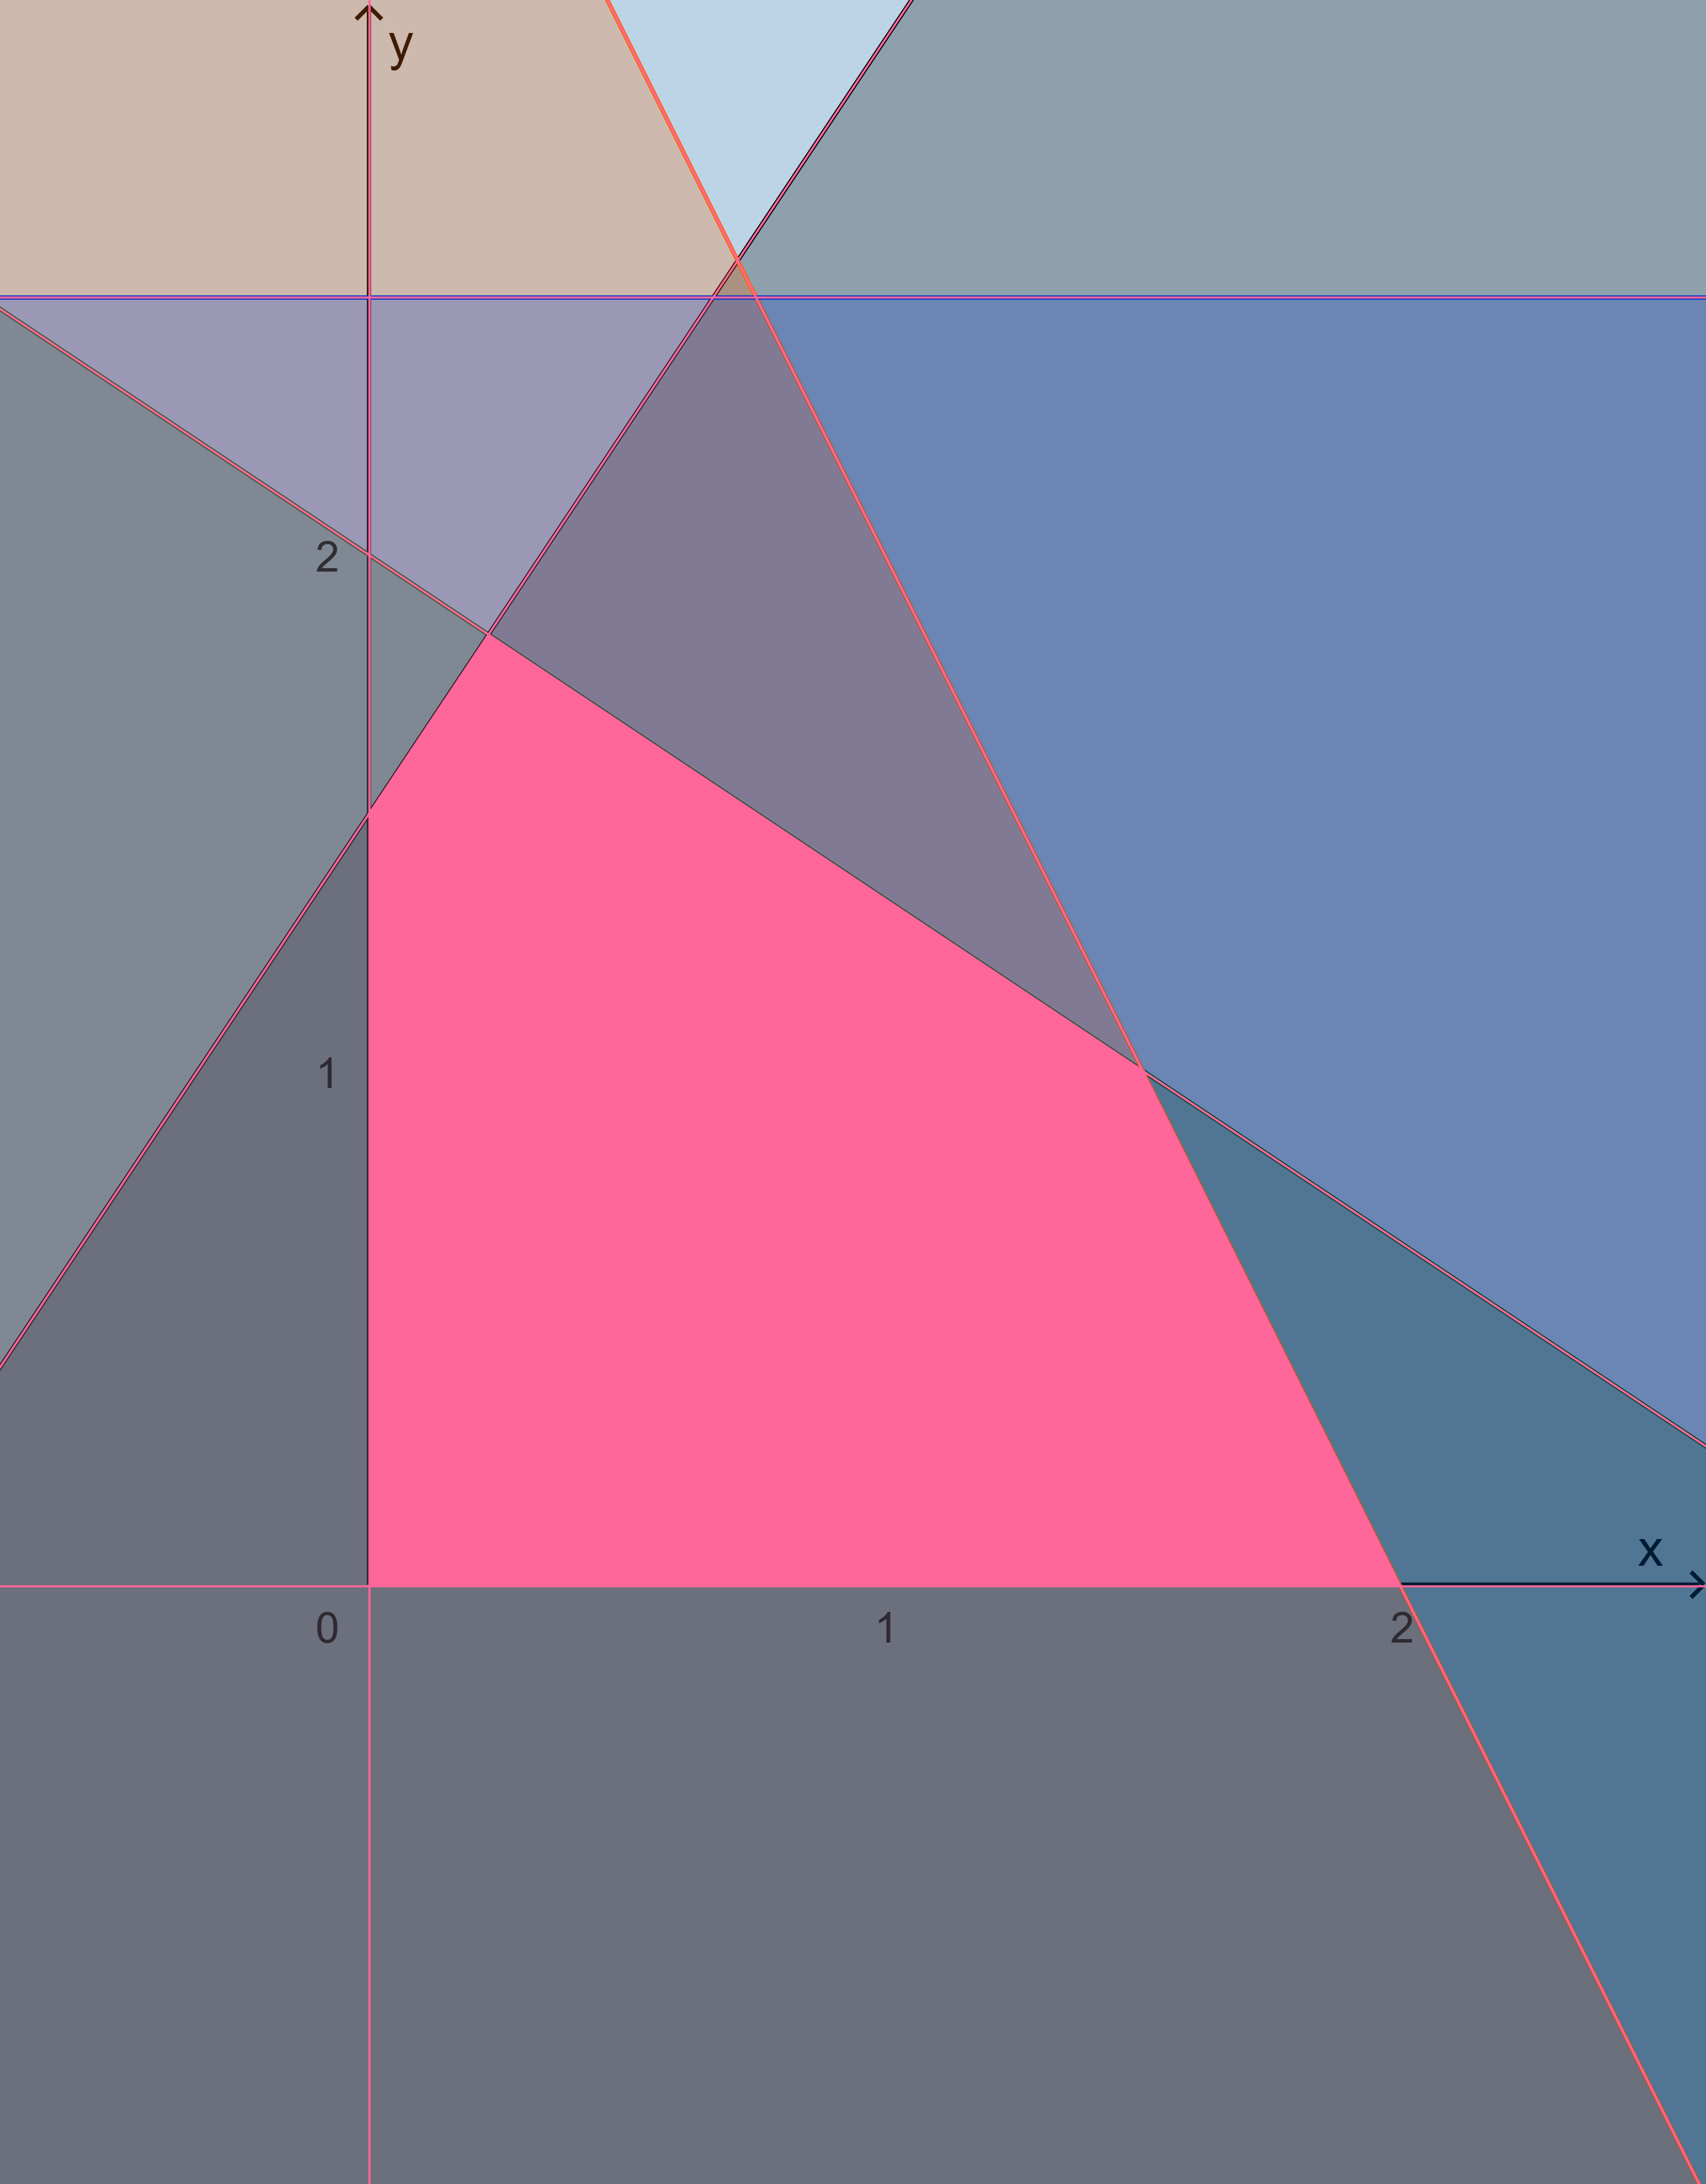
\includegraphics[width=0.5\textwidth]{./figures/ex3-feasible-region.png}
%     \caption{Feasible region for the problems \ref{eq:ex3-min-f}, \ref{eq:ex3-constraints}}
%     \label{fig:feasible-region}
% \end{figure}

% \subsection*{b)}

% The basic feasible points are the vertices of the feasible region described by the polytope
% visible in Figure \ref{fig:feasible-region}.
% The vertices can be computed by solving the system of equations
% following the geometrical interpretation:

% Let \( \vibar{x}{1} := x_1 \geq 0 \; \cap \; x_2 \geq 0 \),
% the result is trivial since \( x_1 = 0 \) is the y-axis
% and \( x_2 = 0 \) is the x-axis,
% so the result is the origin \( O \).
% Anyways, the intersection is computed by solving the system:

% \myex{false}{}{
%     \begin{cases}
%         x_1 = 0 \\
%         x_2 = 0
%     \end{cases}
%     \quad
%     \vibar{x}{1} = \myvec{0 \\ 0} = O
% }

% Let \( \vibar{x}{2} := x_1 \geq 0 \; \cap \; 3 + 3 x_1 - 2 x_2 \geq 0 \).
% The intersection is computed by solving the system:

% \myex{false}{}{
%     \begin{cases}
%         x_1 = 0 \\
%         3 + 3 x_1 - 2 x_2 = 0
%     \end{cases}
%     \Rightarrow
%     \begin{cases}
%         x_1 = 0 \\
%         x_2 = \frac{3}{2}
%     \end{cases}
%     \quad
%     \vibar{x}{2} = \myvec{0 \\[3pt] \frac{3}{2}}
% }

% Let \( \vibar{x}{3} := 3 + 3 x_1 - 2 x_2 \geq 0 \; \cap \; 6 - 2 x_1 - 3 x_2 \geq 0 \).
% The intersection is computed by solving the system:

% \myex{false}{}{
%     \begin{cases}
%         3 + 3 x_1 - 2 x_2 = 0 \\
%         6 - 2 x_1 - 3 x_2 = 0
%     \end{cases}
%     \Rightarrow
%     \begin{cases}
%         x_1 = \frac{2}{3} x_2 - 1 \\
%         x_2 = \frac{24}{13}
%     \end{cases}
%     \quad
%     \vibar{x}{3} = \myvec{\frac{3}{13} \\[6pt] \frac{24}{13}}
% }

% Let \( \vibar{x}{4} := 6 - 2 x_1 - 3 x_2 \geq 0 \; \cap \; 4 - 2 x_1 - x_2 \geq 0 \).
% The intersection is computed by solving the system:

% \myex{false}{}{
%     \begin{cases}
%         6 - 2 x_1 - 3 x_2 = 0 \\
%         4 - 2 x_1 - x_2 = 0
%     \end{cases}
%     \Rightarrow
%     \begin{cases}
%         x_2 = 1 \\
%         4 - 2 x_1 - (1) = 0
%     \end{cases}
%     \quad
%     \vibar{x}{4} = \myvec{\frac{3}{2} \\[3pt] 1}
% }

% Let \( \vibar{x}{5} :=  4 - 2 x_1 - x_2 \geq 0 \; \cap \; x_2 \geq 0 \).
% The intersection is computed by solving the system:

% \myex{false}{}{
%     \begin{cases}
%         4 - 2 x_1 - x_2 = 0 \\
%         x_2 = 0
%     \end{cases}
%     \Rightarrow
%     \begin{cases}
%         4 - 2 x_1 - (0) = 0 \\
%         x_2 = 0
%     \end{cases}
%     \quad
%     \vibar{x}{5} = \myvec{2 \\ 0}
% }

% To find the optimal point \( \mathbf{x}^* \) that minimizes \( f \) subject to the constraints,
% we evaluate the function \( f \) at each vertex of the polytope in the feasible region:

% \myex{false}{}{
%     f(\vibar{x}{1}) &= 4 \cdot 0 + 3 \cdot 0 &&= 0 \\[3pt]
%     f(\vibar{x}{2}) &= 4 \cdot 0 + 3 \cdot \frac{3}{2} &&= \frac{9}{2} \\[3pt]
%     f(\vibar{x}{3}) &= 4 \cdot \frac{3}{13} + 3 \cdot \frac{24}{13} &&= \frac{84}{13} \\[3pt]
%     f(\vibar{x}{4}) &= 4 \cdot \frac{3}{2} + 3 \cdot 1 &&= 9 \\[3pt]
%     f(\vibar{x}{5}) &= 4 \cdot 2 + 3 \cdot 0 &&= 8
% }

% The optimal point \( \mathbf{x}^* \) that minimizes \( f \) subject to the constraints
% is the point \( \mathbf{\overline{x}_1} \) vertex of the polytope in the feasible region.

% \myex{false}{}{
%     \arg \min_{\mathbf{x} \in \mathcal{\overline{X}} }
%     f(\mathbf{x}) = \vibar{x}{1}
%     \qquad \mathcal{\overline{X}}
%     = \{
%     \vibar{x}{1},
%     \vibar{x}{2},
%     \vibar{x}{3},
%     \vibar{x}{4},
%     \vibar{x}{5}
%     \}
% }

% \subsection*{c)}

% To prove that the first order necessary conditions hold for the optimal points,
% we need to verify the KKT conditions from (\ref{eq:ex2-kkt})
% for the optimal point \( \vibar{x}{1} = \myvec{0 & 0}^T \).
% The active set \( \mathcal{A}( \vibar{x}{1} ) = \{ 5, 6 \} \)
% where the constraints \( c_5 := x_2 \geq 0 \) and \( c_6 := x_1 \geq 0 \)
% from (\ref{eq:ex3-constraints}) are active, both \( c_5, c_6 = 0 \therefore \)
% the point \( \vibar{x}{1} \) is at a polytope vertex.
% By checking the LICQ condition, the gradients of the active constraints are linearly independent:

% \myex{false}{}{
%     \langle \nabla c_5, \nabla c_6 \rangle
%     =
%     \langle \myvec{0 \\ 1}, \myvec{1 \\ 0} \rangle
%     =
%     0
% }

% Find \( \lambda_5, \lambda_6 \):

% \myex{false}{}{
%     \nabla f = \myvec{4 \\ 3}, \quad
%     \nabla c_5 = \myvec{0 \\ 1}, \quad
%     \nabla c_6 = \myvec{1 \\ 0} \\
%     \myvec{4 \\ 3} = \lambda_5 \myvec{0 \\ 1} + \lambda_6 \myvec{1 \\ 0}
%     \Rightarrow
%     \begin{cases}
%         \lambda_6 = 4 \\
%         \lambda_5 = 3
%     \end{cases}
% }

% Finally, let's check that the gradient of the Lagrangian function is zero at the optimal point
% \( \mathbf{x}^* = \vibar{x}{1} \),
% as rewritten in (\ref{eq:ex2-computed-complementary-condition}):

% \myex{false}{}{
%     \nabla_{x} \mathcal{L}(\mathbf{x}^*, \lambda^*)
%     &= \nabla f - \sum_{i \in \mathcal{A}( \mathbf{x}^* )} \lambda_i^* \nabla c_i \\
%     &= \myvec{4 \\ 3} - 3 \myvec{0 \\ 1} - 4 \myvec{1 \\ 0} \\
%     &= \myvec{0 \\ 0} = \mathbf{0}
% }

% Hence, the first order necessary conditions hold for the optimal point \( \vibar{x}{1} \).


\end{document}
